\chapter{Work Completed}
	\section{Data Accumulation}
		We used dataset created during a Deepfake Image Detection and Reconstruction
		Challenge. Two datasets of real face images were used: CelebA and FFHQ. Various
		Deepfake images were generated using architectures such as StarGAN, GDWCT,
		AttGAN, StyleGAN, and StyleGAN2. Specifically, CelebA images were manipulated
		using pre-trained models available on GitHub for StarGAN, GDWCT, and AttGAN.
		Images from StyleGAN and StyleGAN2 created through FFHQ were obtained. A sample of real and fake images are shown below:

	\begin{figure}[hbt!]
		\centering
		\begin{minipage}{0.45\textwidth}
				\centering
				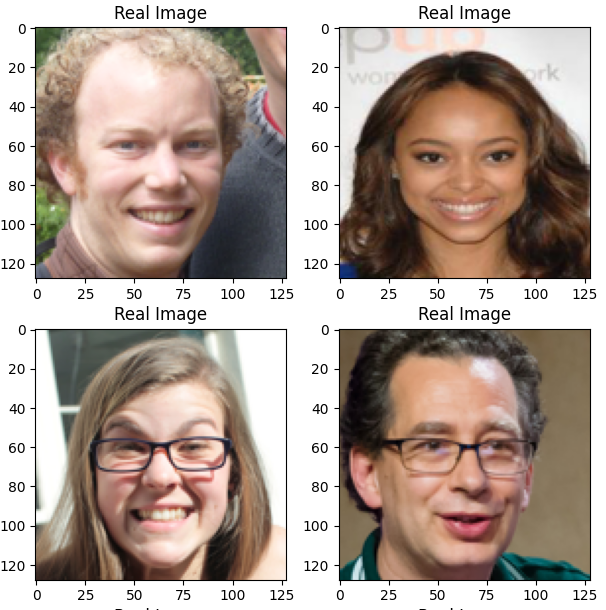
\includegraphics[width=0.95\linewidth]{./img/real sample.png}
				\caption{Real Images}
		\end{minipage}
		\hfill
		\begin{minipage}{0.45\textwidth}
				\centering
				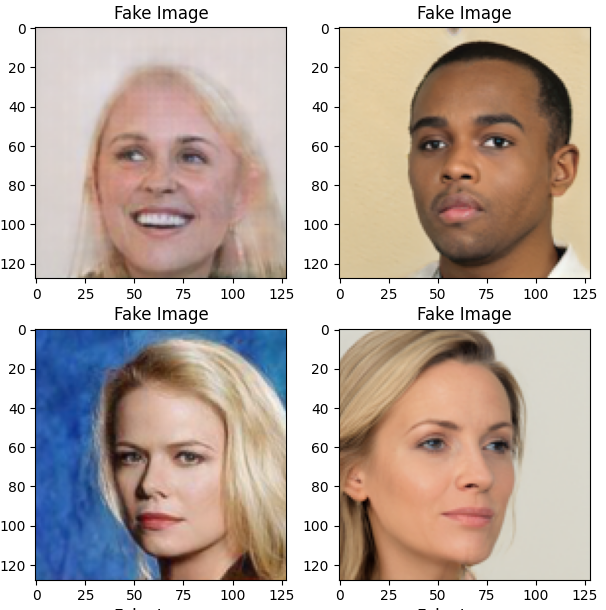
\includegraphics[width=0.95\linewidth]{./img/fake sample.png}
				\caption{Fake Images}
		\end{minipage}
	\end{figure}

	\section{Data Preprocessing}
	\subsection{Data Augmentation}
		To balance our dataset, we augmented our images to achieve a total of 25000 images for each category. For the 5000 fake images, we applied four different transformations, resulting in 20000 augmented fake images. For the real images, we randomly selected and transformed 3750 images, generating 15000 augmented real images. Various transformations, such as rotation, compression, scaling, and mirroring, were implemented. A sample of each transformation is shown below:

	\begin{figure}[hbt!]
		\centering
		\begin{minipage}{0.45\textwidth}
				\centering
				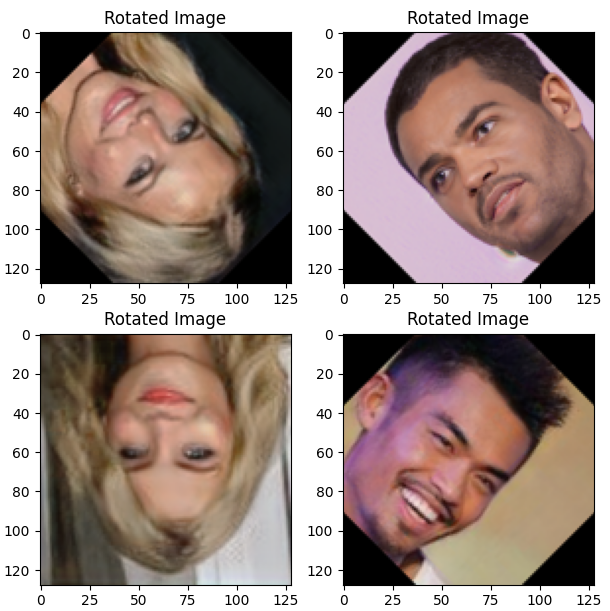
\includegraphics[width=0.95\linewidth]{./img/rotated.png}
				\caption{Rotated Images}
		\end{minipage}
		\hfill
		\begin{minipage}{0.45\textwidth}
				\centering
				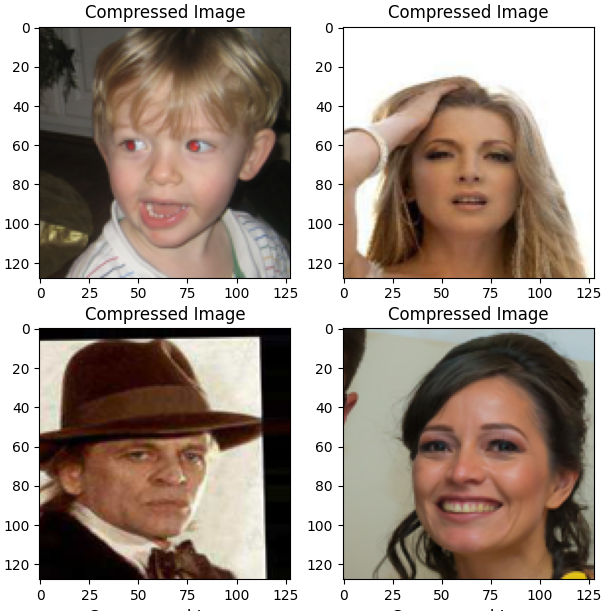
\includegraphics[width=0.95\linewidth]{./img/compressed.png}
				\caption{Compressed Images}
		\end{minipage}

		\vspace{0.5cm} % Add some vertical space between the two rows of images

		\begin{minipage}{0.45\textwidth}
				\centering
				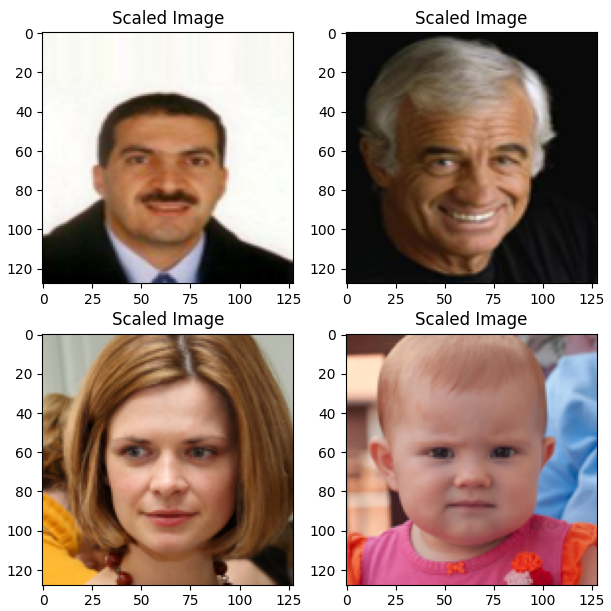
\includegraphics[width=0.95\linewidth]{./img/scaled.png}
				\caption{Scaled Image}
		\end{minipage}
		\hfill
		\begin{minipage}{0.45\textwidth}
				\centering
				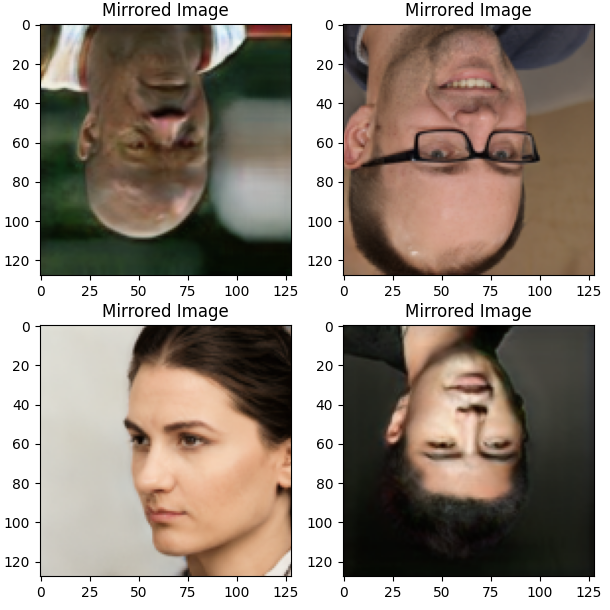
\includegraphics[width=0.95\linewidth]{./img/mirrored.png}
				\caption{Mirrored Images}
		\end{minipage}
	\end{figure}

	\subsection{Data Normalization}
	First, we computed the mean and standard deviation of the entire dataset, which consists of both the original dataset and the augmented dataset. The normalization process was then applied using the following formula:
	\begin{equation}
	x = \frac{x - \mu}{\sigma}
	\end{equation}
	where \(x\) represents the pixel values of each image pixel.
	
	This approach standardizes the features to have a mean of 0 and a standard deviation of 1. This standardization is crucial because certain machine learning algorithms are sensitive to the scale of the input features.

	\subsection{Data Splitting}
	We partitioned our dataset into a training set, comprising 80\% of the dataset, and a validation set, consisting of 20\% of the dataset. This division ensures that the model has an ample amount of data for learning, while also offering a subset of the data to assess the model's performance.

	\section{Setting Parameters}
	\begin{itemize}
		\item \textbf{Number of epochs : 50} \\
			The number of epochs refers to the number of times the complete training dataset is passed through the network during the training process. Each epoch consists of one forward pass (input to output) and one backward pass (error calculation and weight updates) for all the training samples.
		\item \textbf{Loss function : Cross-Entropy} \\
			Loss function is a method of evaluating how well your algorithm models your dataset. Cross-entropy loss measures the difference between a deep learning classification model's discovered and predicted probability distributions.

			The cross-entropy between two probability distributions, such as q from p, can be stated formally as
			
			\begin{equation}
				H(p, q) = -\sum_{x \in \mathcal{X}} p(x) \log q(x)
			\end{equation}

			Where
			\begin{itemize}
				\item H is the cross-entropy function
				\item p may be the target distribution
				\item q is the approximation of the target distribution.
			\end{itemize} 

		\item \textbf{Learning rate : 0.001} \\
			The learning rate is a hyperparameter that determines the step size at which an optimization algorithm.
		\item \textbf{Optimizer : Adam} \\
			An optimizer  is an algorithm used to update the parameters (weights and biases) of a model during training in order to minimize the loss function. 
			Adam (short for Adaptive Moment Estimation) is a popular optimization algorithm known for its robustness, efficiency, and ease of use. It often converges faster and performs better than traditional optimization algorithms.
			It adapts the learning rate for each parameter individually based on the past gradients and squared gradients making it well suited for training models.
	\end{itemize}

	\section{Model Training}
